\documentclass[12pt,twoside, a4paper, twocolumn]{article}
\usepackage[utf8]{inputenc}
\usepackage[brazil]{babel}
\usepackage[margin = 0.5in]{geometry}
\usepackage{amsmath}
\usepackage{amsthm}
\usepackage{amssymb}
\usepackage{amsthm}
\usepackage{setspace}
\usepackage[americanvoltages,fulldiodes,siunitx]{circuitikz}
\usepackage{lipsum}
\usepackage{pgfplots}
\usepackage{ifthen}
\usepackage{adjustbox}
\usepackage[section]{placeins}
\usepackage{hyperref}
\usepackage{graphicx}
\usepackage{amsmath}
\usepackage{amsthm}
\usepackage{amssymb}
\usepackage{amsthm}
\usepackage{setspace}
\usepackage[americanvoltages,fulldiodes,siunitx]{circuitikz}
\usepackage{lipsum}
\usepackage{pgfplots}
\usepackage{ifthen}
\usepackage{adjustbox}
\usepackage[section]{placeins}
\usepackage{hyperref}
\usepackage{graphicx}
\usepackage{adjustbox}
\usepackage{indentfirst}




\pgfplotsset{compat=newest}
\graphicspath{ {./images/} }
%  #1 color - optional #2 x_0 #3 y_0 #4 x_f #5 y_f #6 name - optional  #7 true if adding lines to axis
\newcommand{\drawvector} [9] [color=cyan] {
\draw[line width=1.5pt,#1,-stealth](axis cs: #2, #3)--(axis cs: #4, #5) node[anchor=south west]{$#6$};
\ifthenelse{\equal{#7}{true}}{
\draw[line width=1pt,#1, dashed](axis cs: #4, #5)--(axis cs: #4, 0) node[anchor= north west]{$#8$};
\draw[line width=1pt,#1, dashed](axis cs: #4, #5)--(axis cs: 0, #5) node[anchor=south east]{$#9$};
}
{}
}
\newcommand\deriv[2]{\frac{\mathrm d #1}{\mathrm d #2}}
\title{Quinto Relatório de Lab de Circuitos II}
\author{Henrique da Silva \\ hpsilva@proton.me}
\date{\today}
\pgfplotsset{width = 10cm, compat = 1.9}
\begin{document}
\maketitle
\pagenumbering{gobble}
\newpage
%pagenumbering{roman}
\tableofcontents
\newpage


\section{Introdução}


Neste relatório, vamos discutir quadripolos, e vamos projetar, montar e testar um quadripolo simples, obtendo seus parâmetros \emph{Z}.




Todos arquivos utilizados para criar este relatório, e o relatorio em si estão em:  \url{https://github.com/Shapis/ufpe_ee/tree/main/5th semester/Circuits II/}


\section{Análise preliminar}


Utilizarei o Maxima para fazer a análise teórica do circuito antes de montá-lo fisicamente.




Após terminar as análises compararei os resultados obtidos nas análises numéricas e em laboratório para verificar sua coerência.


\subsection{O circuito}


\begin{figure}[h]
    \centering
    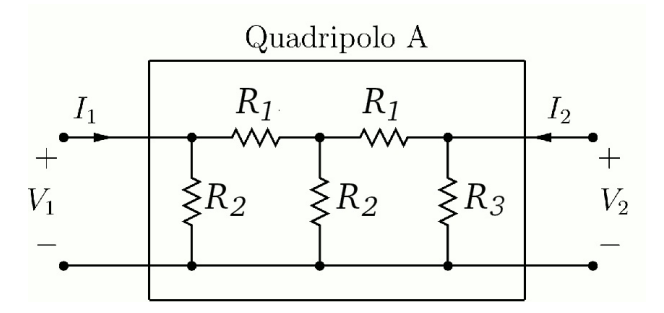
\includegraphics[width=1\columnwidth]{images/circuito.png}
    \caption{Quadripolo puramente resistivo.}
\end{figure}




\pagebreak
\subsection{Maxima}


Podemos realizar a análise do circuito utilizando análise nodal.


\begin{equation}
    \begin{aligned}
         & {{\mathrm{V_1}-\mathrm{V_a}}\over{\mathrm{R_1}}}+{{\mathrm{V_1}}\over{
        \mathrm{R_2}}}-\mathrm{I_1}=0                                             \\
         & {{\mathrm{Va}-\mathrm{V_2}}\over{\mathrm{R_1}}}+{{\mathrm{Va}-
        \mathrm{V_1}}\over{\mathrm{R_1}}}+{{\mathrm{V_a}}\over{\mathrm{R_2}}}=0   \\
         & {{\mathrm{V_2}-\mathrm{V_a}}\over{\mathrm{R_1}}}+{{\mathrm{V_2}}\over{
        \mathrm{R_3}}}-\mathrm{I_2}=0                                             \\
    \end{aligned}
\end{equation}


\paragraph*{}
Resolvendo simbolicamente no Maxima obtemos o seguinte:




\begin{figure}[h]
    \centering
    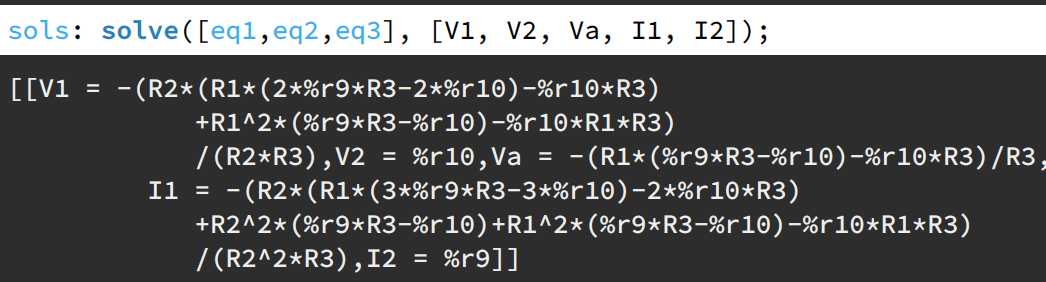
\includegraphics[width=1\columnwidth]{images/solve.png}
    \caption{Resolvendo o sistema da análise nodal  para $V_1$, $V_2$, $V_a$, $I_1$ e $I_2$.}
\end{figure}


Com estas soluções em mãos podemos obter os parâmetros \emph{Z} do circuito.


Para isto vamos obter cada um individualmente, zerando a corrente $I_1$ e $I_2$ em cada caso onde aplicável.


\begin{figure}[h]
    \centering
    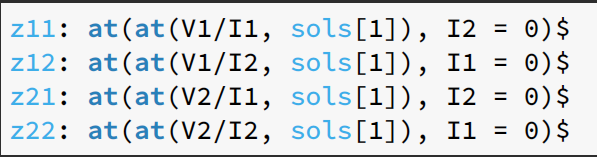
\includegraphics[width=1\columnwidth]{images/parametrosZ.png}
    \caption{Obtendo parâmetros Z.}
\end{figure}


\begin{equation}
    \begin{aligned}
         & Z_{11} = 21343.6125 \\
         & Z_{12} = 15333.9925 \\
         & Z_{21} = 15333.9925 \\
         & Z_{22} = 23826.6225 \\
    \end{aligned}
\end{equation}




Com estes em mãos podemos obter a total impedância do circuito com uma carga $Z_L$ aplicada na sua saída.


Para isto vamos substituir os valores dos resistores, e daí podemos dividir a tensão de entrada pela corrente de entrada e obter a impedância do circuito.




\begin{figure}[h]
    \centering
    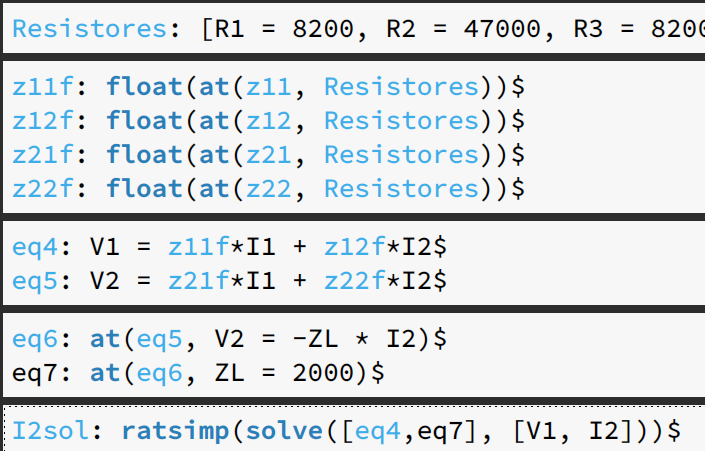
\includegraphics[width=1\columnwidth]{images/ZL.png}
    \caption{Obtendo $V_1$ e $I_2$ para impedancia de carga $Z_L = 2000$.}
\end{figure}




Agora com $V_1$, $V_2$, $I_1$ e $I_2$ em mãos podemos obter a total impedância do circuito.


\begin{equation}
    Z_{in} = \frac{V_1}{I_1} = 12239.38973 \varOmega
\end{equation}




\section{Medições em laboratório}


\subsection{O quadripolo}




Inicialmente farei as medições dos componentes a serem usados.


Após isso montarei os circuitos e realizei as medições de tensão e corrente, com estes obterei os parâmetros $Z$ do circuito.


E por fim, medir a impedância total do circuito para confirmar que os resultados que obtive são coerentes


\subsection{Tabela de componentes}




\subsubsection*{Quadripolo A}
\begin{equation}
    \begin{aligned}
        R_{11} & = 8.18k \varOmega  \\
        R_{12} & = 8.2k \varOmega   \\
        R_{21} & = 46.37k \varOmega \\
        R_{22} & = 46.87k \varOmega \\
        R_{3}  & = 81.66k \varOmega \\
        Z_L    & = 1.95 \varOmega
    \end{aligned}
\end{equation}


\subsection{Resultados das medidas}


\paragraph*{Para $I_1 = 0$}
\begin{center}
    \begin{tabular}{ |c|c|c|c| }
        \hline
        Grandezas & $I_1 = 0$     & $I_2 = 0$     & Com  $Z_L$    \\
        $V_1$     & $0.647 V$     & $1.01 V$      & $1.01$        \\
        $V_2$     & $1.01 V$      & $0.725 V$     & $0$           \\
        $I_1$     & $0$           & $47.37 \mu A$ & $82.15 \mu A$ \\
        $I_2$     & $42.00 \mu A$ & $0$           & $0$           \\


        \hline
    \end{tabular}
\end{center}


\pagebreak


\subsection{Parâmetros \emph{Z}}


\begin{equation}
    \begin{aligned}
         & Z_{11} = 21321.5115052 \\
         & Z_{12} = 15404.7619048 \\
         & Z_{21} = 15305.0453874 \\
         & Z_{22} = 24047.6190476 \\
    \end{aligned}
\end{equation}




\subsection{Com resistência de entrada}


\begin{equation}
    \begin{aligned}
         & V_1 = 1.01 V                           \\
         & I_1 = 82.15 \mu A                      \\
         & R_{in} = 12294.5830797 \varOmega       \\
         & R_{in} esperado = 12239.3897 \varOmega \\
    \end{aligned}
\end{equation}




\section{Conclusões}




Conseguimos com sucesso fazer a análise numérica pelo Maxima, e comparamos os resultados com os obtidos experimentalmente.




Nos resultados práticos, obtivemos parâmetros $Z$ bastante similares aos obtidos numericamente.


E também uma impedancia total de circuito bastante semelhante como podemos observar em (6).


Em suma creio que tivemos sucesso em nos familiarizar com as ferramentas de análise de circuitos elétricos numéricos, e métodos para análise de quadripolos.


\end{document}